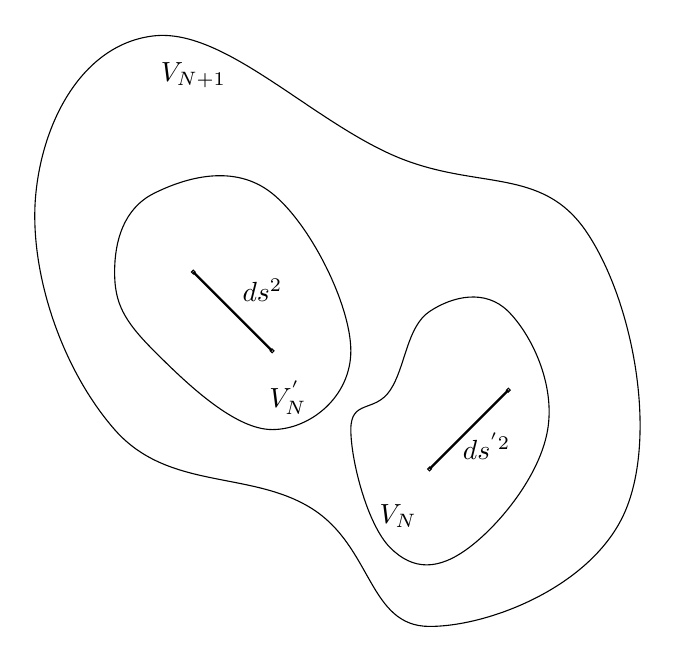
\begin{tikzpicture}
\draw  plot[smooth cycle, tension=.7] coordinates {(-3.5,6.5) (-0.5,5) (2,4) (2.5,0.5) (0,-1) (-1.5,0.5) (-4,1.5) (-5,4.5)};
\draw  plot[smooth cycle, tension=.7] coordinates {(-3.5,4.5) (-2,4.5) (-1,2.5) (-2,1.5) (-3.5,2.5) (-4,3.5)};
\draw  plot[smooth cycle, tension=.7] coordinates {(1,3) (1.5,1.5) (0.5,0) (-0.5,0) (-1,1.5) (-0.5,2) (0,3)};
\node at (-3,6) {$V_{N+1}$};
\node at (-1.8,1.9) {$V^{'}_{N}$};
\node at (-0.4,0.4) {$V_{N}$};
\coordinate (v1) at (-3,3.5) {};
\coordinate (v2) at (-2,2.5) {};
\draw[fill=white](v1) circle(0.7pt)node[{anchor=north }] {};
\draw[fill=white](v2) circle(0.7pt)node[{anchor=north }] {};
\draw[thick]   (v1) -- (v2);
\coordinate (v3) at (1,2) {};
\coordinate (v4) at (0,1) {};
\draw[fill=white](v3) circle(0.7pt)node[{anchor=north }] {};
\draw[fill=white](v4) circle(0.7pt)node[{anchor=north }] {};
\draw[thick]  (v3) -- (v4);
\node at (-2.5,3)[anchor = south west] {$ds^2$};
\node [anchor = south west] at (0.3,1) {$ds^{'2}$};
\end{tikzpicture}\\